\documentclass[conference]{IEEEtran}
\IEEEoverridecommandlockouts
% The preceding line is only needed to identify funding in the first footnote. If that is unneeded, please comment it out.
\usepackage{cite}
\usepackage{amsmath,amssymb,amsfonts}
\usepackage{algorithmic}
\usepackage{graphicx}
\usepackage{textcomp}
\usepackage{xcolor}
\usepackage{optidef}
\def\BibTeX{{\rm B\kern-.05em{\sc i\kern-.025em b}\kern-.08em
    T\kern-.1667em\lower.7ex\hbox{E}\kern-.125emX}}
\begin{document}

\title{Vision-Based Pose Estimation for Launch Vehicle Booster Landing\\
}

\author{\IEEEauthorblockN{Anshuk Chigullapalli}
\IEEEauthorblockA{\textit{Aeronautics and Astronautics} \\
\textit{Stanford University}\\
Stanford, United States \\
anshuk@stanford.edu}
\and
\IEEEauthorblockN{Kristopher Riordan}
\IEEEauthorblockA{\textit{Aeronautics and Astronautics} \\
\textit{Stanford University}\\
Stanford, United States \\
riordk@stanford.edu}
\and
\IEEEauthorblockN{Yuji Takubo}
\IEEEauthorblockA{\textit{Aeronautics and Astronautics} \\
\textit{Stanford University}\\
Stanford, United States \\
ytakubo@stanford.edu}
\and
\IEEEauthorblockN{Faress Zwain}
\IEEEauthorblockA{\textit{Aeronautics and Astronautics} \\
\textit{Stanford University}\\
Stanford, United States \\
fzwain@stanford.edu}
}

\maketitle

\begin{abstract}
A vision-based attitude estimation algorithm for a rocket booster landing is developed. 
In a 3D-rendered world, an AprilTag (ArUcro Marker) placed at the launchpad is utilized as a key landmark of feature detection and matching. 
The measurement is then processed to update a state estimation using the multiplicative extended Kalman filter, where the rotational uncertainty is expressed as a covariance matrix of modified Rodrigues parameters. 
The developed algorithm is validated via a comparison with the IMU-based pose estimation as well as the combined measurement, and the performance of each estimation system is analyzed.  
\end{abstract}

% \begin{IEEEkeywords}
% Pose estimation, Terrain-Relative Navigation, 
% \end{IEEEkeywords}

\section{Introduction}

Reusable rocket boosters are an active point of development in the launch vehicle industry. 
Re-using rocket boosters (i.e. the first stage of a launch vehicle) can significantly reduce the cost of space launch services and increase launch cadence \cite{shotwell2021space}. 
Through these benefits, reusable rockets also make technologies such as in-orbit propellant transfer and long-duration Mars missions economically viable; reliable reusability is a cornerstone of space exploration.

A demonstrated method of retrieving orbital-class boosters is vertical landing with retro-propulsion. 
This has been demonstrated by SpaceX's Falcon 9 and Falcon Heavy (orbital booster) and Blue Origin's New Shepard (sub-orbital booster) \cite{maggio2023vision} \cite{blackmore2016autonomous}. 
As the industry works towards vertical landings with higher precision, such as landing the booster back at the launch pad, a stronger requirement on precise and robust navigation and state estimation algorithm during the final stages of this landing maneuver is desired \cite{blackmore2016autonomous}.

Vision-based estimation has already been demonstrated in space missions such as the Mars 2020 mission \cite{johnson2022mars} or IM-1 lunar lander \cite{christian2021image}, which utilized terrain relative navigation (TRN) for their position estimation and precise autonomous landing. 

This paper evaluates the effectiveness and applicability of the vision-based pose estimation to the booster landing problem. 
One differentiation of the booster landing compared to the planetary landing problem is that we have exact prior knowledge of the landing site and surroundings, while a sub-meter level of navigation accuracy is desired for the pin-point landing. 
In this paper, we further simplify the problem by placing an AprilTag \cite{kallwies2020determining} as a defining landmark for the landing site. 
The pose of the booster is determined by comparing existing onboard camera footage facing the landing pad and pointing to known features at the landing site.
We then process a vision-based pose estimation algorithm with generic IMU-based pose estimation using an Extended Kalman Filter (EKF) to get an improved estimate.  


\section{Related Work}

Image-based localization using cameras can be an effective replacement for time-based filters for highly dynamic systems can result in a loss of information or blur in the dynamics \cite{mair2009efficient}. 
Although a single calibrated camera may achieve an accurate localization, it is best for low-noise measurements with close-range applications.
Reference \cite{mair2009efficient} uses a modified Kanade-Lucas-Tomasi (KLT) tracker for feature tracking and a vision-based GPS for self-estimating the camera poses. 
The image scaling is first initialized using a known feature dimension, structure from motion (SfM), or a stereo camera system with triangulation; then the features are managed at each time step. The algorithm determines whether enough features are trackable to continue high-accuracy pose estimation; if not, the system loops back to KLT to re-initialize features for tracking. 
Experimental results and accuracy comparisons between different models are discussed in more detail \cite{mair2009efficient}.

AprilTags are square tags with distinct monochrome patterns that are commonly used for landmarks of feature detection and estimation algorithms. 
Detailed real-time pose estimation, tracking, and localization in GPS-denied environments and comparisons of the size, accuracy, and speed of several AprilTag implementation algorithms are discussed in Ref. \cite{tola2021real}. 
The high-level design includes grayscale, Gaussian smoothing, gradient magnitude \& direction, and edge detection \& clustering. 
Once a set of candidate quads (four-sided shapes made up of the detected edge segments) is generated, the camera extrinsics problem is solved to extract a rotation and translation of the camera in relation to a frame grounded in the AprilTag itself \cite{olson2011apriltag}. 

Due to the variety of different AprilTag detection libraries available, a research project was conducted to compare the localization accuracy of four commonly used, open-source AprilTag detection libraries \cite{kallwies2020determining}. 
Using a 3D camera simulation from OpenGL, the researchers tested each library's localization accuracy with variable parameters such as tag size, viewing angle, tag rotations, and border occlusion. The authors also explain different localization accuracy improvement methods including edge refinement, corner refinement, tag extensions, and filtering out poor tag detections. 
The conclusion states that ArUco OpenCV is best for computational speed, AprilTags C++ is best for accuracy, and AprilTags 3 is the best for a middle ground \cite{kallwies2020determining}. 

Similar, but opposite to our project, robot localization using images of a moving object has proven to be a successful localization method \cite{lee2003localization}. 
The two main methods are position estimation using image projection of the moving target and then correction through the use of a Kalman filter. 
The simulation and experiments show the Kalman filter's ability to recursively correct the position estimation after an initial estimate from the image projection \cite{lee2003localization}. 
Although the camera frame is fixed and the target is moving relative to the camera, the same algorithms are applicable if the camera is moving relative to a fixed target frame. 

In the case of having no AprilTags, utilizing a known map of generic terrain features becomes necessary. Camera-based TRN falls into a subset of visual odometry problems that estimate an ego-motion and pose by moving camera images \cite{nister2004visual, scaramuzza2011visual}, which is a variant of the structure from motion (SfM) problem.
Since it may not require any prior information about the landscape and the trajectory motion but estimates the agent's odometry purely based on iterative feature-matching and outlier rejections, successful real-world online implementations has been demonstrated \cite{christian2021image}.

The Kalman Filter and its variations are the most common sequential state estimation techniques. 
When using a Kalman Filter to estimate the attitude of a rigid body, the state space must be chosen carefully. 
Although quaternions are a typical attitude representation for spacecraft due to the lack of singularities, a unitary norm constraint ($\|q\|=1$) spawns difficulty in the standard Kalman Filter formulation \cite{markley2003mekf}. 
One solution for this issue is a multiplicative Kalman filter (MKF), which utilizes a state space that is composed of the error rotation between the belief state and an updated attitude. 
This error rotation can be chosen to be one of several unconstrained attitude parameterizations (e.g. Gibbs vector, Modified Rodrigues Parameters, Euler angles). If chosen well, this parameterization yields a simple, first-order formulation of the Kalman Filter \cite{markley2003mekf}.

The guidance problem during rocket descent involves the generation of valid trajectories subject to physically imposed and designer imposed constraints. This problem can be formulated as a convex optimization problem using lossless convexification to eliminate pervasive non-convex dynamics and constraints \cite{malyuta2021convex}. Additionally, assuming that the attitude control dynamics operate on a much faster time-scale than the translational dynamics, the trajectory can be simplified to that of a point mass with three degrees of freedom for which the thrust vector dictates the attitude. Using these simplifications and discretizing the dynamics allows for simple and fast trajectory generation that can be done on-board the descent vehicle, often with just a single call of a convex solver \cite{malyuta2021convex}. 

\section{Methodology}

We propose a fully integrated vision-based pose estimation package that takes in camera information and, utilizing existing map information of the landing site, determines the pose of the vehicle through feature detection and matching.

This will be implemented in a simulated environment that combines Blender, a popular 3D graphics tool, and Python. A pre-determined landing trajectory is generated using the methods described in Section \ref{sec:dynamics}. Then, we acquire a sequence of noised-images from a simulated camera in Blender that follows that pre-determined trajectory. These sequence of images are used in the pose-estimation problem. To simplify the problem, the pose estimates are not used in the loop with guidance and control problem. The vision-based pose estimate will then be fused with a simulated IMU pose estimate, to determine if the added visual odometry information improves the final result. Figure \ref{fig:flow_chart} showcases the information flow of the proposed work.

% insert figure here
\begin{figure}[htbp] \label{fig:flow_chart}
    \centerline{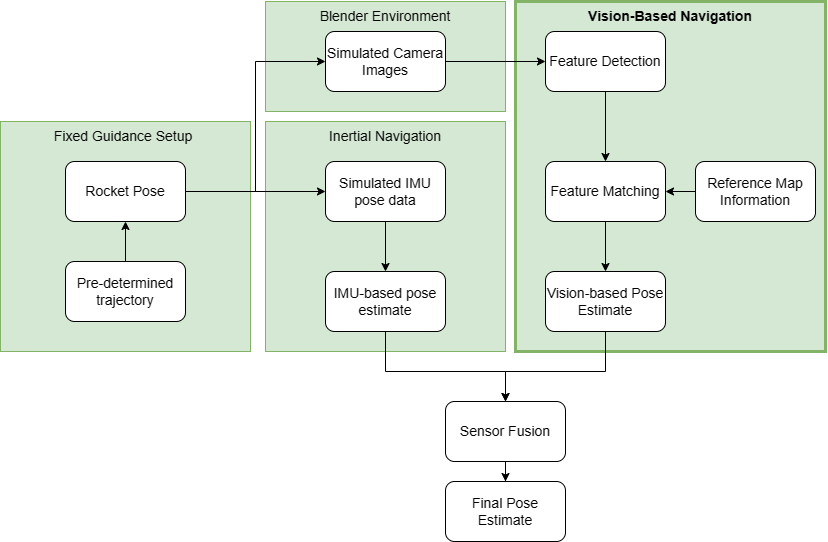
\includegraphics[width=0.49\textwidth]{273_project_flow.png}}
    \caption{Proposed vision-based estimation experiment architecture.}
    \label{fig:sys_arch}
\end{figure}
% insert figure here

\subsection{Vehicle Dynamics and Trajectory Generation} \label{sec:dynamics}

The translational trajectory of the rocket will be generated using a 3-DOF model of the dynamics, treating the vehicle as a point mass. Imposed on the model will be discrete state transition constraints, a pointing constraint, a glide angle constraint, and initial and final conditions set. 
Any non-convexities will be handled using lossless convexification. 
A fuel-optimal trajectory will then be solved for using a convex solver such as CVXPY.
This trajectory will encode a time history of the rocket's position in 3D space along with a thrust vector. It is assumed that the attitude of the booster is equivalent to the thrust vector direction.
From this, a time history of poses will be generated, from which an approximation of instantaneous angular rates can be computed. 
Thus, a full state history of the rocket is made available to feed into the simulated landing environment.
The same tools used on-board landing vehicles to plan and perform powered descent guidance were used to generate a nominal simulation trajectory.
This is done by simplifying the rocket dynamics into a 3-DOF problem with a point mass being acted on by a thrust vector.
The treatment of this problem in continuous time is discussed in detail in Ref. \cite{malyuta2021convex}.
Several constraints in the original formulation of the problem are either non-convex or require changes of variables in order to be DCP compliant.
This leads to what is denoted as Problem 104 in Ref. \cite{malyuta2021convex}, which is cast in continuous time. After discretizing the problem, it can be formulated as is shown in Problem \ref{eq:convex_traj_gen}.

\begin{mini!}|s|[2]<b>{\xi_0, \hdots , \xi_K}{\sum_{k=1}^{K}{\xi_k }\label{eq:objective}}{\label{eq:convex_traj_gen}}{}
\addConstraint{\vec{r}_{k+1}}{= \vec{r}_k + \frac{\delta t}{2} \left( \vec{v}_k + \vec{v}_{k+1} \right)}
\addConstraint{\vec{v}_{k+1}}{= \vec{v}_k + \delta t \left( \vec{u}_k - g\hat{e}_z \right)}
\addConstraint{z_{k+1}}{= z_k - \delta t \alpha \xi_k}
\addConstraint{\mu_{\text{min},k} \left( 1 - \delta z_k + \frac{1}{2} {\delta z_k}^2 \right)}{\leq \xi_k}
\addConstraint{\mu_{\text{max},k} \left( 1 - \delta z_k \right)}{\geq \xi_k}
\addConstraint{\Vert \vec{u}_k \Vert }{\leq \xi_k}
\addConstraint{\vec{u}_k \hat{e}_z^T}{\geq \xi_k \cos{\gamma_{p,k}}}
\addConstraint{\vec{r}_k^T \hat{e}_z}{\geq \gamma_{gs} \Vert H_{gs} \vec{r}_k \Vert}
\addConstraint{\ln{(m_{\text{dry}})}}{\leq z_K}
\addConstraint{z_1}{= \ln{(m_{\text{wet}})}}
\addConstraint{z_{l,k}}{\leq z_k}
\addConstraint{z_k}{\leq z_{u,k}}
\addConstraint{\vec{r}_1}{= \vec{r}_0}
\addConstraint{\vec{r}_K}{= \vec{r}_f}
\addConstraint{\vec{v}_1}{= \vec{v}_0}
\addConstraint{\vec{v}_K}{= 0},
\end{mini!}

The design variables are defined as follows:

\begin{eqnarray*}
    \xi_k \triangleq \frac{\sigma_k}{m_k} & \vec{u}_k \triangleq \vec{T}_k & z_k \triangleq \ln{(m_k)}
\end{eqnarray*}

Parameters such as wet-mass, dry-mass, and specific impulse were chosen to be representative of a rocket similar in size and performance to the first stage of the Falcon 9.
These are listed below.

\begin{eqnarray*}
    I_{sp} = 282 \text{ s} & m_{wet} = 42.2 \cdot 10^3 \text{ kg} & m_{dry} = 22.2 \cdot 10^3 \text{ kg} \\
    \gamma_{gs} = 0.5 \text{ rad} & g = 9.807 \text{ m/s\textsuperscript{2}} & \delta t = 0.1 \text{ s} \\
    t_f = 8 \text{ s}
\end{eqnarray*}

For the purposes of this analysis, no process noise has been injected onto the nominal trajectory. Therefore, the true state of the system is equivalent to the nominal trajectory solution. 

\begin{figure}
    \centering
    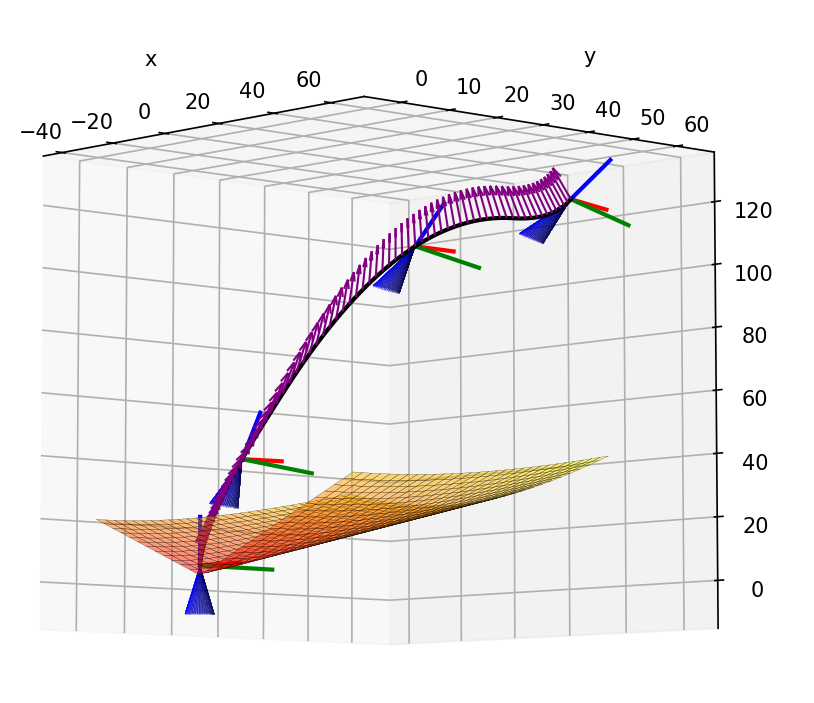
\includegraphics[width=0.5\textwidth]{rocket_traj.png}
    \caption{Reference (True) Landing trajectory with camera attitude.}
    \label{fig:enter-label}
\end{figure}


\subsection{Simulation Environment}
Since it is not feasible to have a physical replica of a vehicle following a booster-like trajectory, a simulation environment is created in Blender to gather images from the perspective of the camera mounted on the booster. The simulated environment has an approximate landing pad and tower, along with a floating camera.

The Blender API allows us tis used to command this floating camera to specific poses in the Blender environment. WI
The pre-determined trajectory timeseries from Section \ref{sec:dynamics} is programmed in Python. The 
At each time step, the simulated pose of the rocket is used as the pose of the camera in Blender. This connection between the Python script and Blender is done using the Blender Python API. The generated camera images are fed back to the Python script, where they will be processed to gather pose estimates.  

% insert figure here
\begin{figure}[htbp] \label{fig:flow_chart}
    \centerline{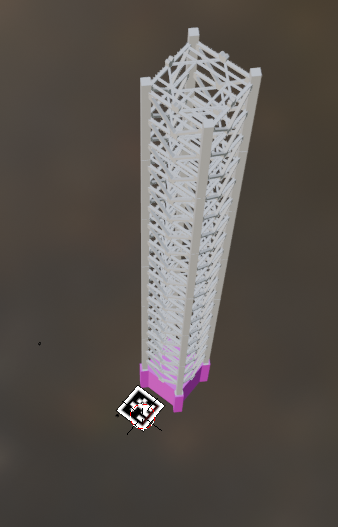
\includegraphics[width=0.3\textwidth]{april_tag_on_booster.png}}
    \caption{Example camera output of a simulated environment in Blender that includes a landing tower with an AprilTag.}
    \label{fig:sys_arch}
\end{figure}
% insert figure here

\subsection{Image Processing}

To simplify the problem, the assumption is made that the landing pad will have a feature-rich ArUco marker, with known feature dimensions (for the real problem, this will just be extended to utilize the 3-dimensional features of the landing pad itself). 
The generated image of the environment (that includes the ArUco marker) at each time step is used to extract the camera's pose. 
With the fully defined camera intrinsic properties and the perfect knowledge of the location of ArUco features, extracting the pose is reduced to solving the camera extrinsics problem. 
The OpenCV library is used for the feature detection and matching algorithm for this implementation.
To briefly discuss the specifics of the OpenCV library's functions, first we used a built in function to detect the ArUco marker's corners and local coordinate frame. 
We confirm that the marker detection was done correctly by plotting the corners and axes on each image. 
The figure below illustrates the detected ArUco marker for a specific time step in our rocket's trajectory.

% insert figure here
\begin{figure}[ht!] 
    \centerline{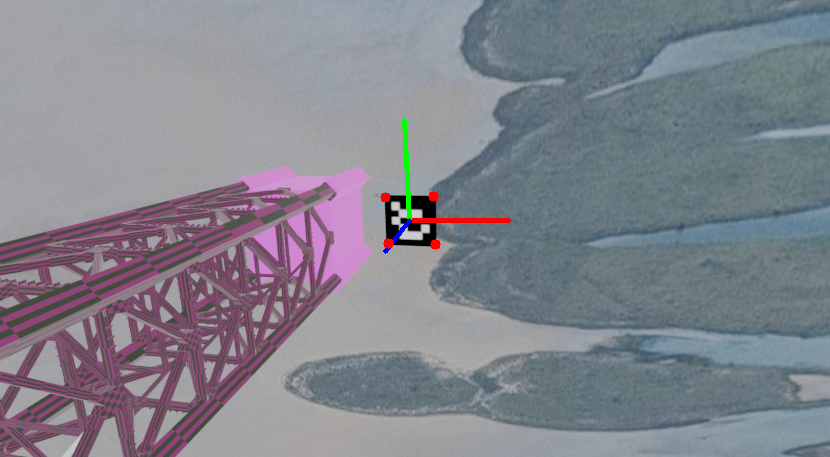
\includegraphics[width=0.4\textwidth]{detectedMarker.png}}
    \caption{Detected ArUco Marker with Defined Corners and Coordinate Frame.}
    \label{fig:marker_}
\end{figure}
% insert figure here

With camera pose now known relative to the world frame as well as relative to the body frame of the rocket, we can extract the rocket pose. 
The camera intrinsic matrix was generated using defined parameters from the blender simulation.

\[
K = \begin{bmatrix}
424.3378 & 0 & 424.0 \\
0 & 424.3378 & 240.0 \\
0 & 0 & 1 \\
\end{bmatrix}
\]

With the ArUco marker simulated with a 10 meter side length in Blender, the origin of the marker's frame as well as its coordinates are known in 3D space. 
The 2D pixel coordinates of the origin and corners are found by OpenCV's detection function. 
The 3D known coordinates coupled with the 2D pixel coordinates allow the PnP problem to be solved with OpenCV's pose estimation function, yielding the camera pose.
The resulting pose is then converted to OpenCV convention then transformed into the world frame to account for the landing pad offset from the actual ground.
The following 


\subsection{Attitude filtering}

The filtering of the rotational motion is executed by a multiplicative extended Kalman filter (MEKF) \cite{markley2003mekf} by choosing a state vector composed of pose error (i.e., error Modified Rodrigues Parameters (MRPs)) and angular velocity in a body frame.
As an error MRPs do not have a unitary norm constraint like a quaternion, computation of the covariance matrix in MRP space simplifies the computation. 
The kinematics of the error MRPs are linearized along the reference quaternion history (i.e., $\delta \boldsymbol{p}^{-}(t) = 0$), where the a posteriori estimate of the error MRP is then used to update the reference quaternion ($\boldsymbol{q}_{\text{ref}}^{k+1}(t) = \delta \boldsymbol{q}(\delta \boldsymbol{p}^{+}(t)) \circ \boldsymbol{q}_{\text{ref}}^k(t)$). 


The prediction step is expressed as follows:
%
\begin{align*}
    q_{t|t+1} & = f(q_{t|t}, \omega_{t|t}, u_t) \\
     \begin{bmatrix}
         \delta p_{t|t+1} \\ \omega_{t|t+1}
     \end{bmatrix} 
     & = A_{t} 
     \begin{bmatrix}
         \delta p_{t|t} \\ \omega_{t|t}
     \end{bmatrix} + B_t u_t  \\
    \Sigma_{t|t+1} & = A_t \Sigma_{t|t} A_t^T + Q_t 
\end{align*}

The update step is expressed as follows:
%
\begin{align*}
    K_t & =  \Sigma_{t+1|t} C_t^\top (C_t \Sigma_{t+1|t} C_t^T + R_t)^{-1} \\
    \begin{bmatrix}
         \delta p_{t+1|t+1} \\ \omega_{t+1|t+1}
     \end{bmatrix}
     & = 
     \begin{bmatrix}
         \delta p_{t|t+1} \\ \omega_{t|t+1}
     \end{bmatrix} + K_t \left(y_t - g\left(\mu_{t+1|t} \right) \right) 
     \\
     \Sigma_{t+1|t+1} & = \Sigma_{t+1|t} - K_t C_t  \Sigma_{t+1|t}  \\
    q_{t+1|t+1} & = \delta q(\delta p_{t}) \circ q_{t+1|t}
\end{align*}

After the update, 

\subsection{Result Validation and Sensor Fusion}
To validate the camera-based pose estimate and determine whether it is a viable method for pose estimation for the booster landing problem, the visual estimate is benchmarked against inertial navigation, i.e. pose estimation using data from an Inertial Measurement Unit. 
As inertial navigation is the current standard method for pose estimation on launch vehicles, it would be useful to validate whether fusing the vision-based pose estimate with the inertial pose estimate provides an improved final result. 


\section{Results}

\subsection{Visual Navigation Results}

\subsection{Vision Denied Case}

\subsection{Vision Enhanced Case}



\section{Conclusion}

% \section*{Acknowledgment}




\bibliographystyle{ieeetr}
\bibliography{reference}

\end{document}
